
\documentclass[border=8pt, multi, tikz]{standalone} 
\usepackage{import}
\subimport{../layers/}{init}
\usetikzlibrary{positioning}
\usetikzlibrary{3d} %for including external image 

\def\ConvColor{rgb:yellow,5;red,2.5;white,5}
\def\ConvReluColor{rgb:yellow,5;red,5;white,5}
\def\PoolColor{rgb:red,1;black,0.3}
\def\UnpoolColor{rgb:blue,2;green,1;black,0.3}
\def\FcColor{rgb:blue,5;red,2.5;white,5}
\def\FcReluColor{rgb:blue,5;red,5;white,4}
\def\SoftmaxColor{rgb:magenta,5;black,7;white,7} 
\def\BSoftmaxColor{rgb:magenta,5;black,7} 
\def\FullyConnected{rgb:blue,2;green,1;white,1}  
\def\BFullyConnected{rgb:blue,2;green,1;black,0.3} 
\def\SumColor{rgb:blue,5;green,15}

\newcommand{\copymidarrow}{\tikz \draw[-Stealth,line width=0.8mm,draw={rgb:blue,4;red,1;green,1;black,3}] (-0.3,0) -- ++(0.3,0);}

\begin{document}
\begin{tikzpicture}
\tikzstyle{connection}=[ultra thick,every node/.style={sloped,allow upside down},draw=\edgecolor,opacity=0.7]
\tikzstyle{copyconnection}=[ultra thick,every node/.style={sloped,allow upside down},draw={rgb:blue,4;red,1;green,1;black,3},opacity=0.7]

\node[canvas is zy plane at x=0] (input) at (-4.2,0,0) {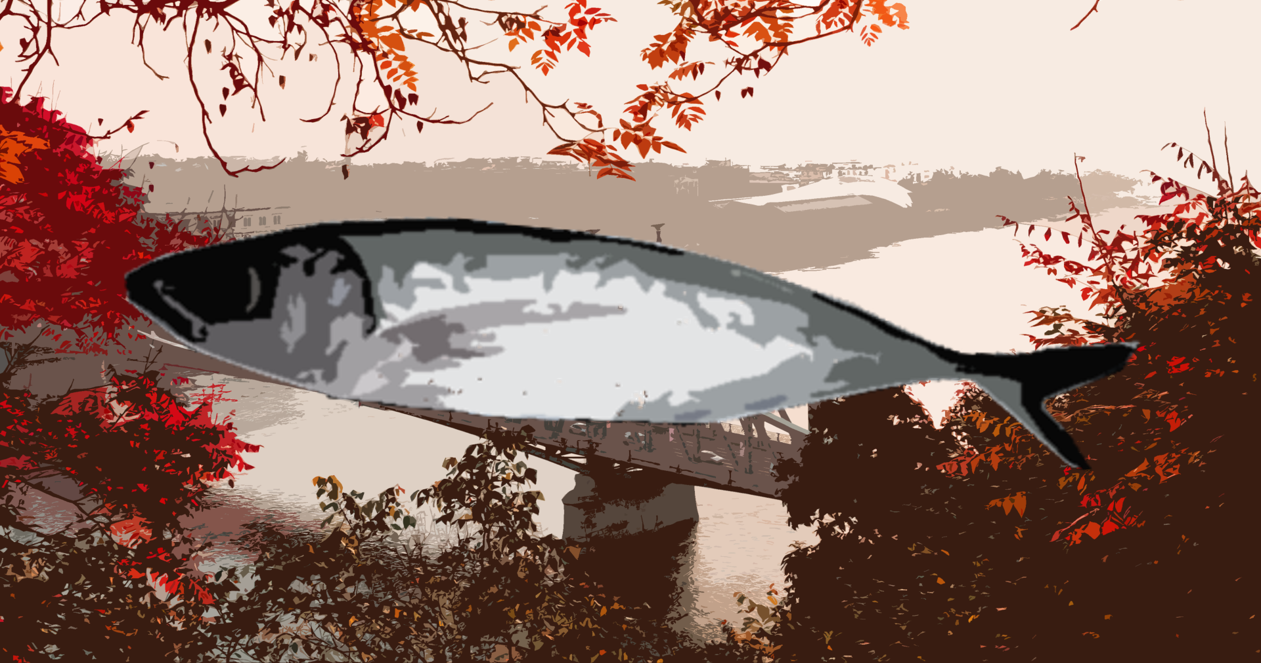
\includegraphics[width=10cm,height=10cm]{fish.png}};

\pic[shift={ (0,0,0) }] at (0,0,0) 
    {RightBandedBox={
        name=conv1_1,
        caption=Conv 1,
        xlabel={{ 64, 64 }},
        ylabel=256,
        fill=\ConvColor,
        bandfill=\ConvReluColor,
        height=40,
        width={ 2 , 2 },
        depth=40
        }
    };

\pic[shift={ (0,0,0) }] at (conv1_1-east) 
    {Box={
        name=pool1,
        caption= ,
        fill=\PoolColor,
        opacity=0.5,
        height=20,
        width=1,
        depth=20
        }
    };

\pic[shift={ (2,0,0) }] at (pool1-east) 
    {RightBandedBox={
        name=conv2_1,
        caption=Conv 2,
        xlabel={{ 128, 128 }},
        ylabel=128,
        fill=\ConvColor,
        bandfill=\ConvReluColor,
        height=30,
        width={ 3 , 3 },
        depth=30
        }
    };

\pic[shift={ (0,0,0) }] at (conv2_1-east) 
    {Box={
        name=pool2,
        caption= ,
        fill=\PoolColor,
        opacity=0.5,
        height=16,
        width=1,
        depth=16
        }
    };

\draw [connection]  (pool1-east)    -- node {\midarrow} (conv2_1-west);

\pic[shift={ (2,0,0) }] at (pool2-east) 
    {RightBandedBox={
        name=conv3_1,
        caption=Conv 3,
        xlabel={{ 256, 256, 256 }},
        ylabel=64,
        fill=\ConvColor,
        bandfill=\ConvReluColor,
        height=25,
        width={ 4 , 4, 4 },
        depth=25
        }
    };

\pic[shift={ (0,0,0) }] at (conv3_1-east) 
    {Box={
        name=pool3,
        caption= ,
        fill=\PoolColor,
        opacity=0.5,
        height=12,
        width=1,
        depth=12
        }
    };

\draw [connection]  (pool2-east)    -- node {\midarrow} (conv3_1-west);

\pic[shift={ (2,0,0) }] at (pool3-east) 
    {RightBandedBox={
        name=conv4_1,
        caption=Conv 4,
        xlabel={{ 512, 512, 512 }},
        ylabel=32,
        fill=\ConvColor,
        bandfill=\ConvReluColor,
        height=20,
        width={ 6 , 6, 6 },
        depth=20
        }
    };

\pic[shift={ (0,0,0) }] at (conv4_1-east) 
    {Box={
        name=pool4,
        caption= ,
        fill=\PoolColor,
        opacity=0.5,
        height=8,
        width=1,
        depth=8
        }
    };

\draw [connection]  (pool3-east)    -- node {\midarrow} (conv4_1-west);

\pic[shift={ (2,0,0) }] at (pool4-east) 
    {RightBandedBox={
        name=conv5_1,
        caption=Conv 5,
        xlabel={{ 512, 512, 512 }},
        ylabel=16,
        fill=\ConvColor,
        bandfill=\ConvReluColor,
        height=15,
        width={ 5 , 5, 5 },
        depth=15
        }
    };

\pic[shift={ (0,0,0) }] at (conv5_1-east) 
    {Box={
        name=pool5,
        caption= ,
        fill=\PoolColor,
        opacity=0.5,
        height=6,
        width=1,
        depth=6
        }
    };

\draw [connection]  (pool4-east)    -- node {\midarrow} (conv5_1-west);

\pic[shift={ (2,0,0) }] at (pool5-east) 
    {RightBandedBox={
        name=fc6,
        caption=FC 1,
        xlabel={1 },
        zlabel=512,
        fill=\FullyConnected,
        bandfill=\BFullyConnected,
        opacity=0.8,
        height=2,
        width={2 },
        depth=40
        }
    };

\draw [connection]  (pool5-east)    -- node {\midarrow} (fc6-west);

\pic[shift={(2,0,0)}] at (fc6-east) 
    {RightBandedBox={
        name=soft1,
        caption=SoftMax,
        xlabel={{" ","dummy"}},
        zlabel=4,
        fill=\SoftmaxColor,
        bandfill=\BSoftmaxColor,
        opacity=0.8,
        height=2,
        width=2,
        depth=10
        }
    };

\draw [connection]  (fc6-east)    -- node {\midarrow} (soft1-west);

\end{tikzpicture}
\end{document}
